\documentclass[a4paper,11pt]{article}
\usepackage[american]{babel}
\usepackage[utf8]{inputenc}
\usepackage{geometry}
\usepackage[ruled,vlined]{algorithm2e}
 \usepackage{algpseudocode}
\usepackage{booktabs}  
\usepackage{graphicx} 
\usepackage{listings}
\usepackage{ragged2e}
\usepackage{syntax}
\usepackage{float}
\usepackage{caption}
\usepackage{subcaption}
\lstset{%
backgroundcolor=\color{cyan!10},
basicstyle=\ttfamily,
numbers=left,numberstyle=\scriptsize
}

\usepackage[wby]{callouts}
\begin{document}

%PORTADA

\begin{titlepage}
\centering
{\includegraphics[width=0.45\textwidth]{/home/juane99/UGR/logo.png}\par}
\vspace{1cm}
{\bfseries\LARGE Escuela T\'ecnica Superior de Ingenier\'ia Inform\'atica y Telecomunicaciones \par}
\vspace{1cm}
{\scshape\Large Pr\'actica 1 \par}
\vspace{1 cm}
{\itshape\Large Memoria Descriptiva Individual \par}
\vspace{1 cm}
{\slshape\Large Juan Emilio Mart\'inez Manj\'on \par}
{\slshape\Large 77024428-G \par}
{\slshape\Large juanemartinez@correo.ugr.es \par}
{\slshape\Large Grupo 4 Martes 11:30h \par}
\vspace{1 cm}
{\bfseries\Large 2019-2020 \par}

\end{titlepage}

%INDICE
\renewcommand{\contentsname}{\bfseries\LARGE\'Indice\vspace{1 cm}}
\tableofcontents

\newpage

%RESTO 

\section{Primeras ideas}

\vspace{5 mm}

Al saber que el tema para la aplicación de este año tenía que girar en torno a la ciudad de Granada, empezamos a proponer ideas. Las primeras ideas que tuvimos tenían que ver con ayudar al cliente a localizar determinados puntos en la cidudad. A continuación expondré mis ideas en aquel momento y como derivaron en lo que es nuestra aplicación hoy en día.

\vspace{5 mm}

Como primera idea se me ocurrió hacer una aplicación que pudiese guiar al cliente por los mejores bares de tapas de Granada. Me pareció una buena idea porque podría ser útil tanto para turistas como para los propios residentes de Granada.

\vspace{5 mm}

Podríamos hacerla para indicar al cliente cuáles son las calles, o las zonas de Granada, donde es mejor la relación calidad-precio de los bares de tapas. Un ejemplo de esto se puede ver en la siguiente imagen:

\vspace{5 mm}

\centering
{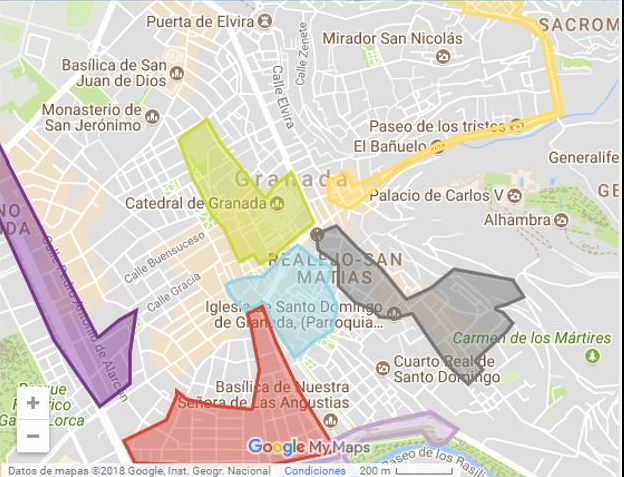
\includegraphics[width=1\textwidth]{imagenes/zonas.png}\par}
\raggedright
\justify

\newpage

Sin embargo, después de darle vueltas me pareció mejor indicar los bares de tapas de forma individual en el mapa. Este cambio se debe a que algunos de los mejores bares de tapas de Granada no están en una calle/zona de tapeo como tal, si no que están en una calle que no se suele relacionar con ese ámbito. Un ejemplo de esto se puede ver en la siguiente imagen:

\vspace{5 mm}

\centering
{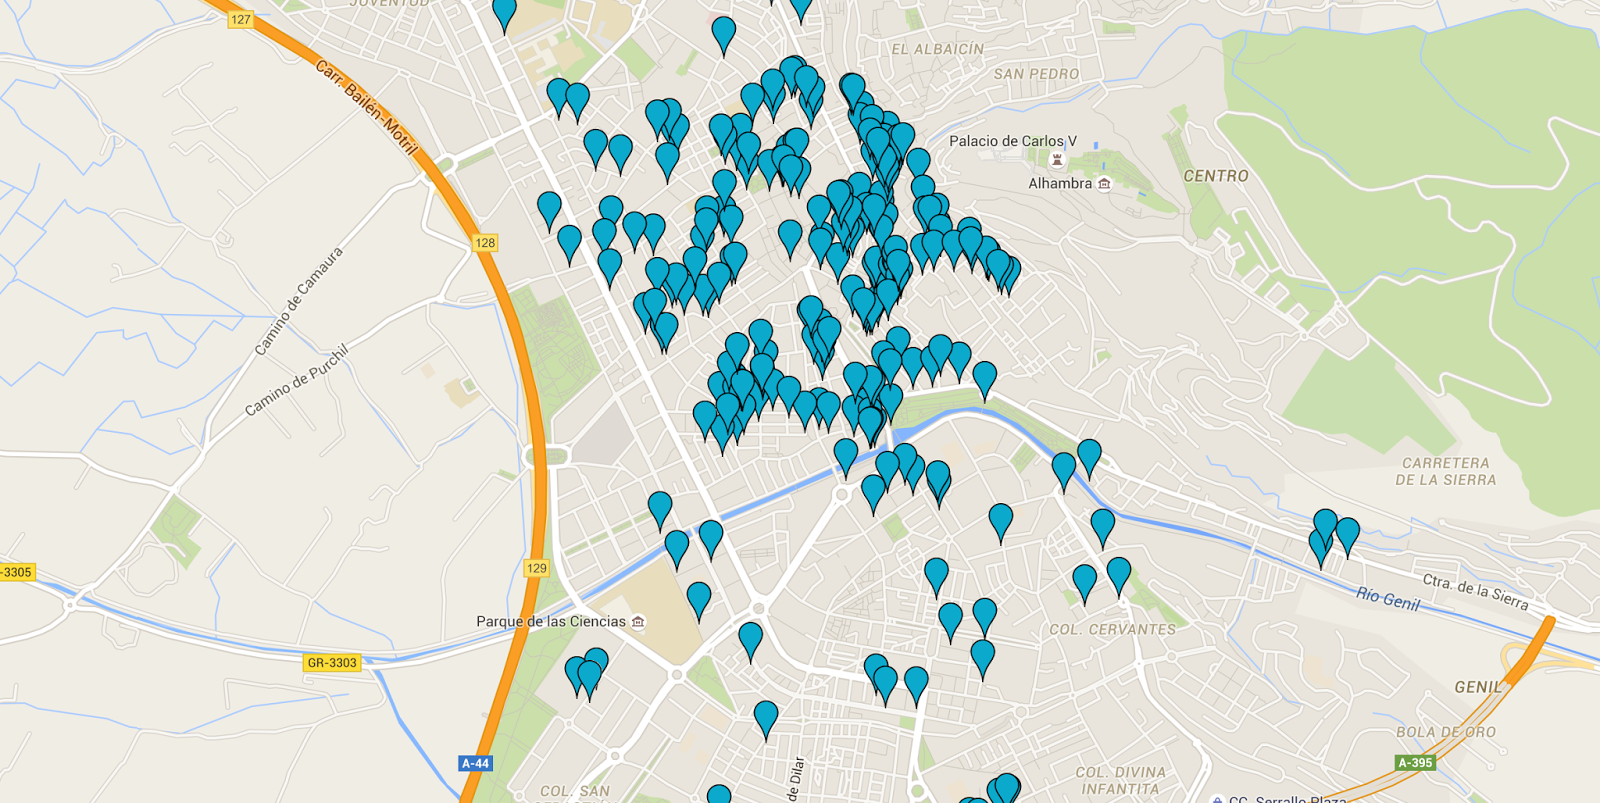
\includegraphics[width=1\textwidth]{imagenes/sitios.png}\par}
\raggedright
\justify

\newpage

\section{Evolución de la idea e integración en la app}

\vspace{5 mm}

Al ver que mis compañeros estaban proponiendo hacer aplicaciones que estuviesen relacionadas con el mundo universitario, se nos ocurrió juntar todas nuestras ideas en una sola aplicación, de tal forma que pudiesemos hacer una \textbf{Guía Universitaria} para cualquier estudiante de la UGR.

\vspace{5 mm}

Por lo tanto, mi idea de los bares de tapas evolucionó de tal forma que no solo mostrase los mejores bares de Granada, si no que mostrase cualquier lugar que pudiese considerarse de interés en Granada. 

\vspace{5 mm}

Es por esto que uno de los apartados del menú de nuestra aplicación se llama \textbf{Sitios de interés}. Al abrirlo veremos un mapa que, con la ayuda de Google Maps, nos muestra los sitios de interés en Granada. A continuación mostraré imágenes de la app:

\vspace{5 mm}

\begin{figure}[H]
\begin{subfigure}{0.41\textwidth}
  \raggedleft
  % include first image
  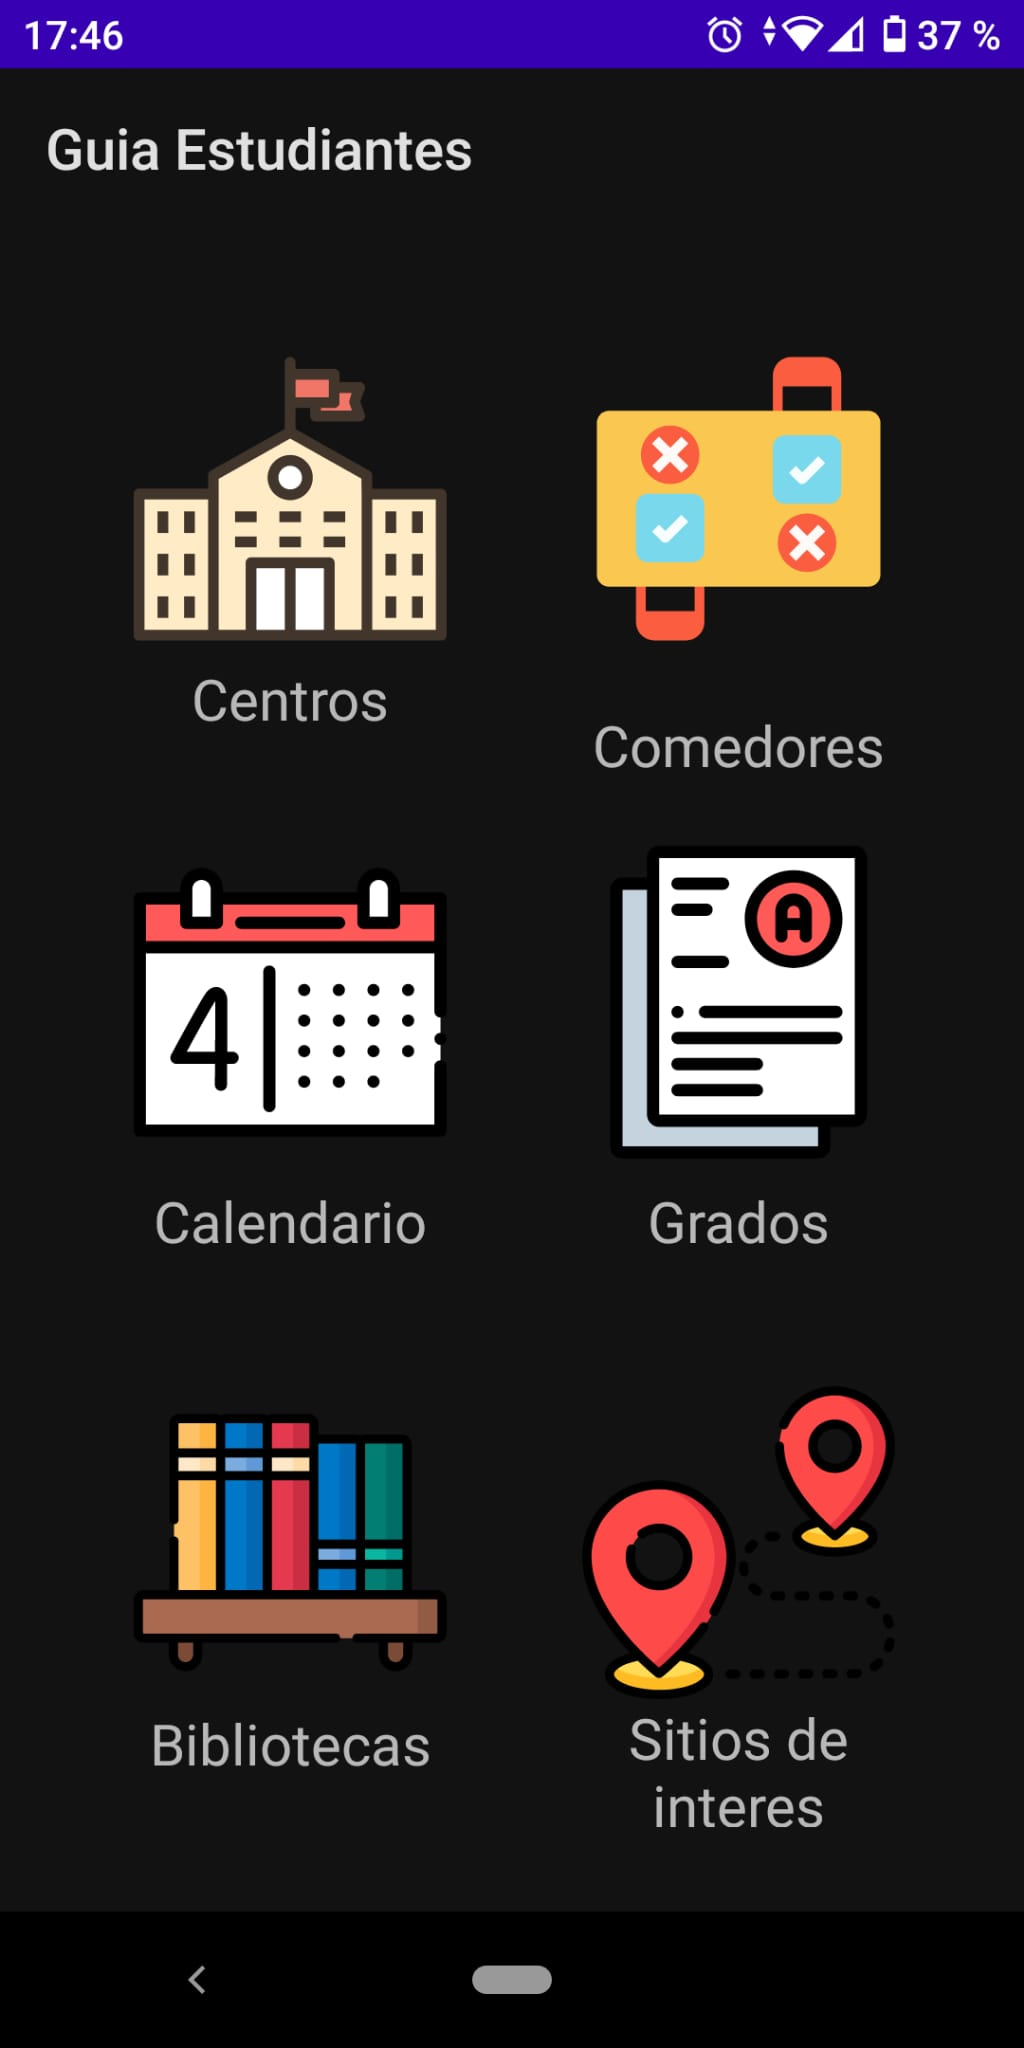
\includegraphics[width=1\linewidth]{imagenes/menu.jpeg}  
  \caption{Menú de la app}
  \label{fig:sub-first}
\end{subfigure}
\hspace{1 cm}
\begin{subfigure}{0.41\textwidth}
  \raggedright
  % include second image
  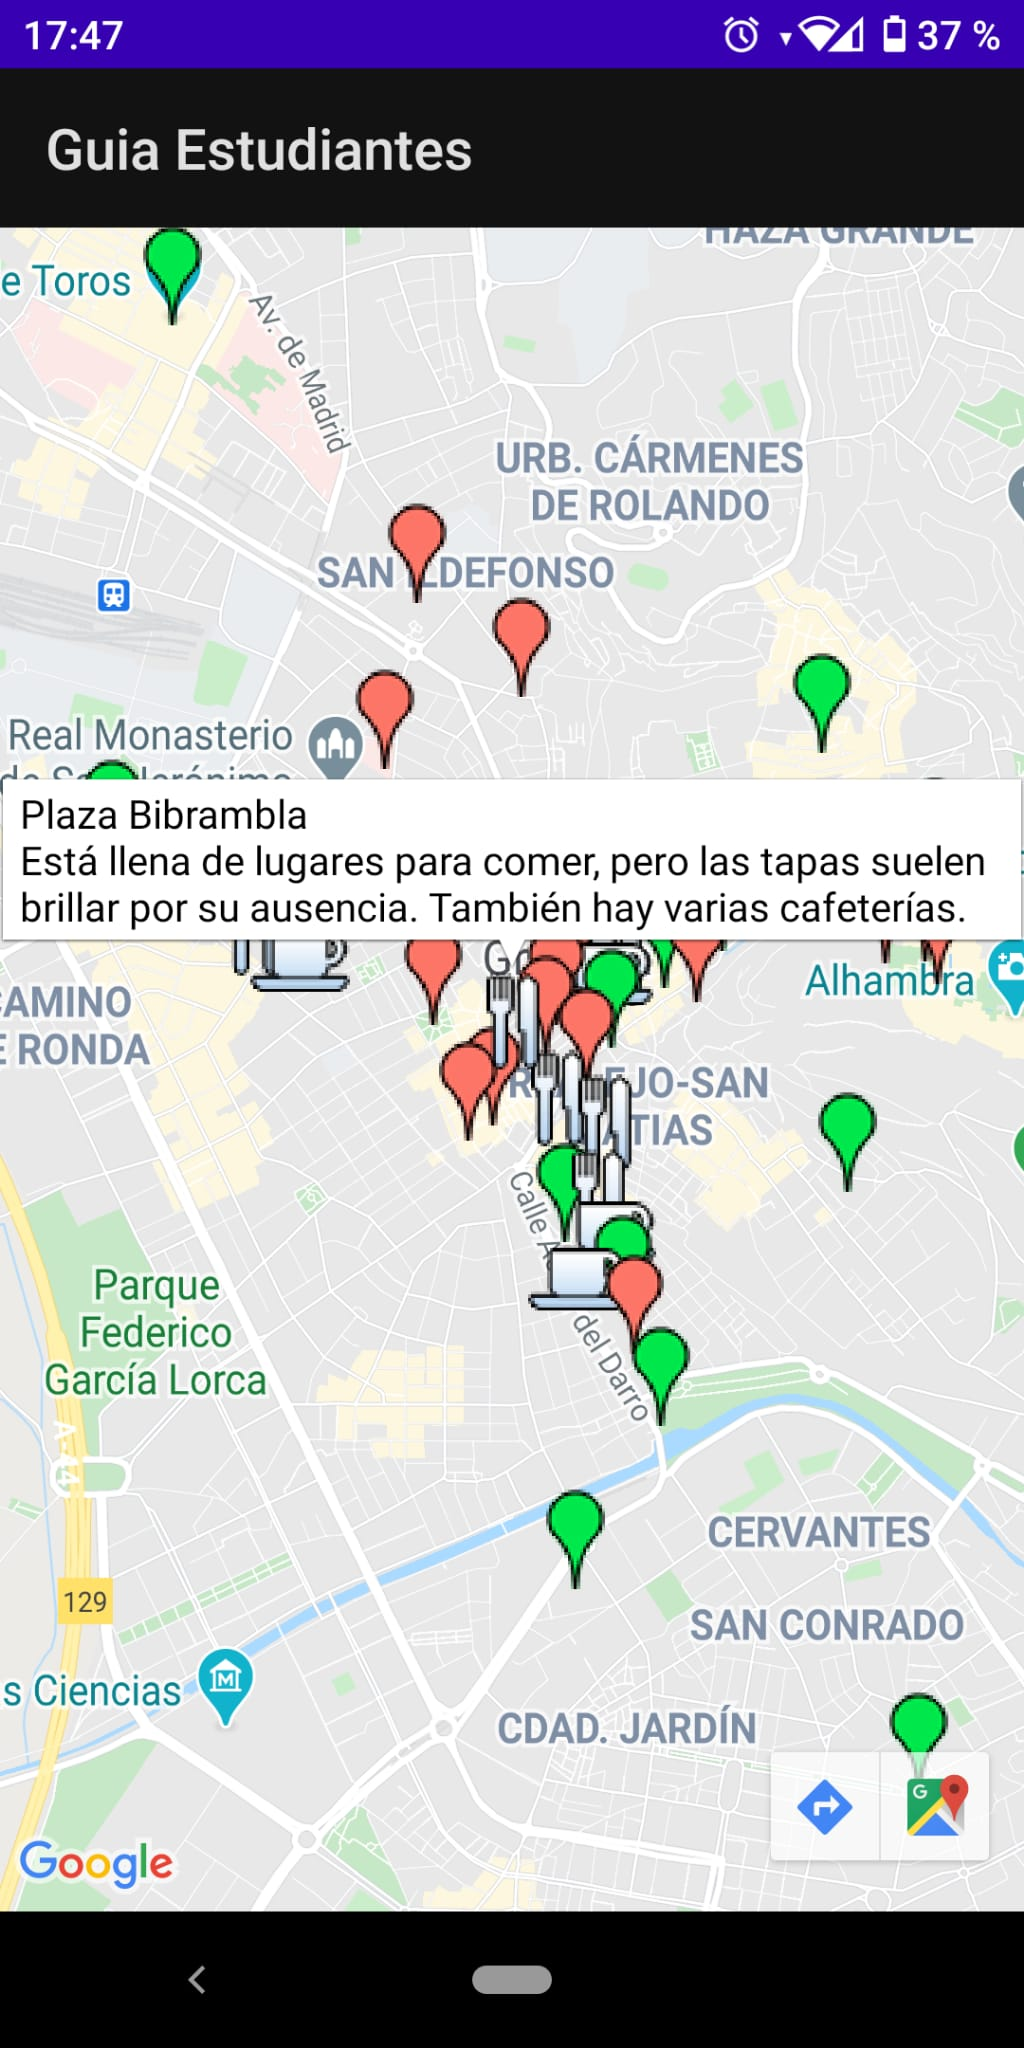
\includegraphics[width=1\linewidth]{imagenes/mapa.jpeg}  
  \caption{Sitios de interés}
  \label{fig:sub-second}
\end{subfigure}
\end{figure}

\end{document}
